\documentclass[a4paper,12pt]{article}
\usepackage{caption}
\usepackage{subcaption}
\usepackage{float}
\usepackage[T1]{fontenc}
\usepackage[italian]{babel}
\usepackage[utf8]{inputenc}
\floatstyle{ruled}
\usepackage{hyperref}
\usepackage{graphicx}
\usepackage{amsmath}
\usepackage{amssymb}
\usepackage[width=125mm]{caption}
\usepackage{amsthm}
\usepackage{algorithm2e}
\usepackage{dsfont}
\usepackage{amsthm}
\usepackage{algpseudocode}
\usepackage{empheq}
\usepackage{tikz}
\usepackage{cancel}

% Dimensione della pagina
\setlength{\oddsidemargin}{.3in}  % Distance from the left edge -1 inch 
\setlength{\textwidth}{145mm}     % Normal width of the text
\setlength{\topmargin}{.25in}     % Distance from top to PAGE'S HEAD -1 inch
\setlength{\textheight}{225mm}    % Height of the body of page
\setlength{\headheight}{0mm}      % Height of a box containing the head
\setlength{\parskip}{0.5mm}         % Extra vertical space before a paragraph
\setlength{\parindent}{9mm}       % Width of the indentation 
\linespread{1.12}                 % Line spacing        
\renewcommand{\floatpagefraction}{.9}



\begin{document}

\title{\bf \Huge Progetto di riparo per il telescopio comunale\\ }


\author{Gruppo Astronomico Città di Seveso\\
Sede Legale: Via Asiago 7/A - Seveso
}


\maketitle
%a
%---------------------------------------------------------
\begin{abstract}
In questa relazione viene presentato il progetto di costruzione di un riparo per il Telescopio Comunale. Si discutono i seguenti punti:
	\begin{itemize}
		\item[1.] Spiegazione delle motivazioni che ci hanno spinto a chiederne la realizzazione;
		\item[2.] Presentazione degli attuali problemi;
		\item[3.] Proposta di realizzazione con le varie specifiche tecniche.
	\end{itemize}
\end{abstract}
%--------------------------------------------------------

%----------------------------------------------------------------------------
\section{Motivazioni}
Dal 2008 il Gruppo Astronomico Citt\`a di Seveso ha prodotto una notevole quantit\`a di dati scientifici di prim'odine. All'attivo abbiamo numerosi dati pubblicati sulle Minor Planet Circular. Queste sono circolari, pubblicate dal Minor Planet Center di Harvard, in cui vengono raccolti i dati scintifici delle pi\`u grandi survay di osservazioni mondiali. I dati vengono direttamente usati dal Jet Propulsion Laboratory (JPL) per stilare le effemeridi di tutti gli oggetti del sistema solare. Oltre agli asterodi abbiamo all'attivo anche un articolo scritto per l'American Association of Variable Stars Observers in cui riportiamo importanti misure di stelle variabili. Abbiamo anche contribuito alla scoperta di una stella variabile e di un esopianeta. Oltre all'attivit\`a scientifica, ci siamo sempre impegnati con energia nella divulgazione didattica a largo spettro. Abbiamo organizzato, gratuitamente, laboratori di astronomia e osservazioni guidate per tutte e tre le scuole medie pubbliche di Seveso. Con cadenza ogni primo venerd\`i del mese (pi\`u eventi particolari come notte di S. Lorenzo) ci siamo sempre aperti verso il pubblico organizzando serate osservative gratuite ad ingresso libero. Da qualche anno a questa parte non riusciamo pi\`u a garantire questi eventi a causa di una serie di problemi che sono descritti nella presente relazione.

\section{Problemi dell'osservatorio}
I problemi dell'osservatorio possono essere divisi in tre categorie principali:
\begin{itemize}
	\item[i.] Problemi legati all'attacco di muffe;
	\item[ii.] Problemi legati alla stabilit\`a del telescopio;
	\item[iii.] Problemi legati alla porzione di cielo visibile dall'attuale sede.
\end{itemize}

\subsection{Problema delle Muffe}
La permanenza a villa Dho, \`e stata sempre fonte di gravissimi problemi di umidit\`e stagnante.Nel piccolo locale messo a nostra disposizione proliferano in modo vorace le muffe. Nonostante la nostra periodica opera di pulizia totale di tutta la strumentazione, spesso troviamo le nostre componenti ottiche in situazioni particolarmente gravi come quelle in Fig.~\ref{FILTRO}. Le muffe ricoprono tutta la superficie ottica cibandosi del trattamento antiriflesso (a base organica) presente. Il continuo ripetersi di queste situazioni sta danneggiando in modo irreparabile tutte le nostre componenti ottiche.
\begin{figure}
	\centering
	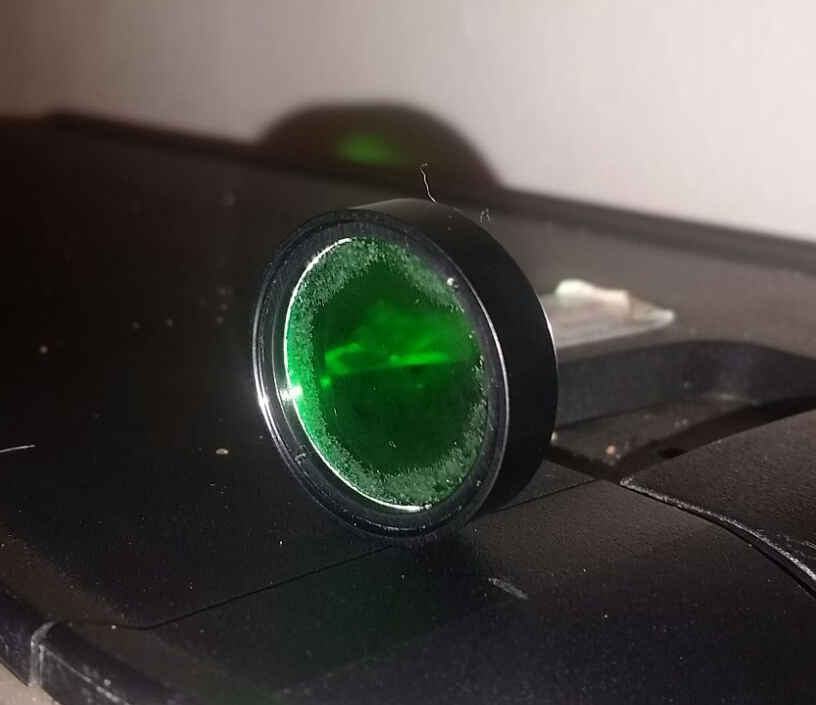
\includegraphics[width=120mm,angle=0,clip=,scale=0.5]{filtro.jpg}
	\caption{Filtro fotometrico attaccato dalle muffe}
	\label{FILTRO}
\end{figure}
\subsection{Problema della stabilit\`a del telescopio}
L'impossibilit\`a di costruire una postazione fissa a Villa Dho, ci costringe a montare/smontare il telescopio ogni serata osservativa. Il suo trasporto manuale, in relazione alla sua mole, rende particolarmente delicata questa operazione. Nonostante tutte le attenzioni del caso, ci sono sempre delle sollecitazioni che col tempo stanno disallineando gli specchi. Il loro riallineamento costa parecchio tempo, con la possibilit\`a che se l'operazione viene ripetuta troppo di frequente, questi si possano danneggiare in modo irreparabile. \`E necessario che il telescopio si trovi in una postazione fissa, senza essere sottoposto a continue sollecitazioni meccaniche.
Oltre al fatto del danneggiamento un ulteriore problema \`e rappresentato dal fatto di non avere un setup stumentale costante nel tempo. Questo problema limita in modo fortissimo i nostri lavori di ricerca in quanto siamo costretti a compiere una riconfigurazione da zero ogni sessione osservativa. La nostra stumentazione ci permetterebbe tranquillamente di collaborare con ulteriori programmi di ricerca (oltre a quelli a cui gi\`a collaboriamo), ma a causa di questi problemi, per ora ci sono preclusi.
\subsection{Problema della Porzione di Cielo}
Oltre al problema della stabilit\`a data dal continuo trasporto e del set-up stumentale non fisso, si aggiunge anche la limitata porzione di cielo visibile da Villa Dho. Gli alberi che sono stati piantati successivamente al nostro arrivo, ora hanno completamente oscurato la porzione di cielo che era visibile.

\section{Soluzione costruzione Riparo}
Dopo una serie di incontri con l'Arch. Bovi, l'Arch. Cappelletti, il Sindaco Butti e la dirigente scolastica Dott.ssa. Parravicini, siamo giunti alla conclusione unanime che le scuole medie di Baruccana sono il posto ideale dove poter posizionare in modo fisso il telescopio comunale. Il progetto che vi presentiamo \`e suddiviso in tre parti principali: la prima parte riguarda l'identificazione, all'interno della scuola, di un locale dove posizionare tre computer per il controllo del nostro telescopio e due armadietti per il nostro materiale, (oculari, fotocamere, filtri ecc ecc...). La seconda parte rigurda l'identificazione della locazione, con le specifiche
della sua realizzazione, del riparo per il telescopio che sar\`a sul tetto della scuola, infine come terzo punto si vuole trattare l'argomento del collegamento tra sala di controllo e telescopio.
\subsection{La sala controllo}
Come concordato con tutti i rappresentati del comune, presenti nel sopralluogo di Gioved\`i 19 Novembre - 2015, la sala di controllo del telescopio sar\`a situata nell'ex aula di informatica (l'aula dei \textit{muretti}) in quanto \`e gi\`a dotata di un ingresso indipendente dalla scuola. Per il nostro utilizzo \`e necessario che questa aula sia dotata di:
\begin{itemize}
	\item Corrente elettrica;
	\item Una scrivania;
	\item Il posto dove poter posizionare i nostri due armadi (mettere misure degli armadi);	\item Un cavo ethernet collegato allo switch principale della scuola.
\end{itemize}

\subsection{Il riparo sul tetto}
Come detto nel precedente paragrafo si propone una struttura minimale che sia in grado di garantire sicurezza e riparo da agenti atmosferici al telescopio. Le modalit\`a di realizzazione che proponiamo sono le seguenti:
\subsubsection{Riparo autocostruito a tetto apribile \textit{a fiore}}
Questa realizzazione \`e sicuramente la pi\`u economica e necessita di:
\begin{itemize}
	\item[->] Un telaio in acciaio in modo da costruire un serramento che si apra dal centro, come visibile in Fig.~\ref{SERR:FIORE};
\begin{figure}
	\centering
	\begin{subfigure}[b]{0.4\textwidth}
		\centering
		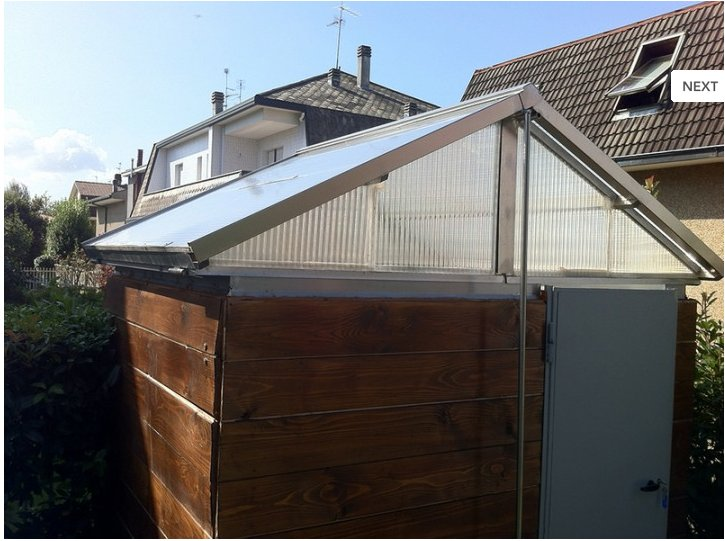
\includegraphics[width=120mm,angle=0,clip=,scale=0.5]{tetto1.jpeg}
		\caption{Struttura di esempio col tetto chiuso}
	\end{subfigure}
	\qquad\quad
	\begin{subfigure}[b]{0.4\textwidth}
		\centering
		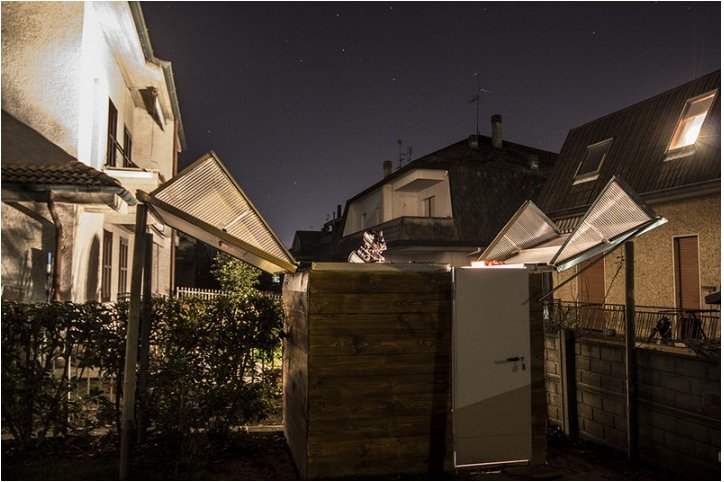
\includegraphics[width=120mm,angle=0,clip=,scale=0.5]{tetto2.jpeg}
		\caption{Struttura di esempio col tetto aperto e i supporti laterali}
	\end{subfigure}
	\caption{Modalit\`a di riparo con apertura a \textit{fiore}}
	\label{SERR:FIORE}
\end{figure}
	\item[->] In Fig.~\ref{SERR:FIORE} il telaio \`e stato riempito con del plexiglass. Nel nostro caso verr\`a saldata una lamiera coibentata.
	\item[->] La struttura del tetto sar\`a posizionata sopra ad un cubo $2m\times2m\times1.50m$
	      che rappresenter\`a la sede del telescopio. La sua realizzazione sar\`a sempre in lamiera coibentata supportata da quattro pilastrini che sorgerebbero ai vertici della base del quadrato.
      \item[->] Per evitare infiltrazioni d'acqua dal pavimento si \`e pensato di realizzare un pavimento in materiale composito, uno strato in legno, uno strato in gomma e nuovamente uno strato in legno. Questo sar\`a fissato con delle ganasce (in modo da non forare il tetto) alle piottole del tetto. Tutta la struttura, oltre ad essere fissata alla sua base, sar\`a fissata ulteriormente, sempre con delle ganasce che si stringono a vite, al corrimano del terrazzo che fa angolo (si veda la pianta Fig.~\ref{PIANTA}). \`E opportuno che il riparo venga dotato anche di una presa d'aria che permetta il flusso d'aria (evitando il ristagno d'aria quindi la formazione delle muffe).`
      \item[->] Al riparo dovr\`a arrivare \textbf{corrente elettrica} e un cavo di collegamento \textbf{ethernet}. La corrente sembra essere accessibile da pi\`u punti in particolar modo da un quadro elettrico gi\`a presente sul terrazzo (sotto ad una grande antenna), rimane da definire bene il persorso che fanno i cavi ethernet gi\`a presenti all'interno della struttura. Da un primo sopralluogo \`e sembrato che sia possibile accedere ad uno switch prossimo al terrazzo.

\end{itemize}
Una stima del prezzo del riparo si aggira intorno ai \textbf{5000euro}.

\subsubsection{Riparo autocostruito a tetto apribile \textit{a scorrimento}}
Gli accorgimenti per il cubo contentente il telescopio sono gli stessi del progetto del riparo con il tetto a fiore. In questo caso cambia la gestione della meccanica di apertura del tetto. 
\begin{itemize}
	\item[->] La costruzione prevederebbe sempre un'intelaiatura in acciaio seguita da una ricopertura in lamiera coibentata. La sua realizzazione dovrebbe essere approssimativamente come in Fig.~\ref{SCORR:TETTO}, con ovviamente i materiali specificati precedentemente.
	\item[->] A differenza della costruzione in Fig.~\ref{SCORR:TETTO} La nostra idea prevede che i supporti dei binari del tetto in modalit\`a aperta, possano essere retratti, abbassati o sgnaciati, una volta che il tetto sia in modalit\`a chiusa.
\begin{figure}
	\centering
	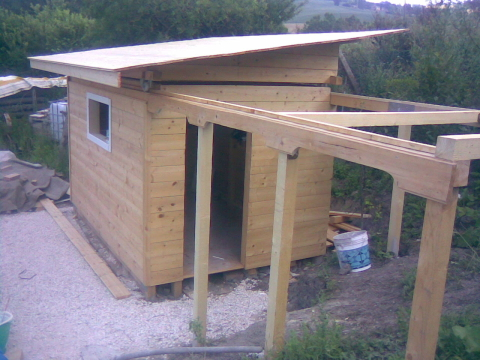
\includegraphics[width=120mm,angle=0,clip=,scale=0.5]{tettoscorr1.jpg}
	\caption{Esempio di struttura a tetto scorrevole. In questo caso l'estensione dei binari esterna \`e fissa. Nel nostro caso, i binari per supportare il tetto aperto, sarebbero richiudibili o sganciabili una volta che il tetto viene chiuso}
	\label{SCORR:TETTO}
\end{figure}
\end{itemize}

Una stima del prezzo di questo ripato si aggira intorno ai \textbf{7000euro}. 

\subsubsection{Cupola remotizzata Avalon}
Esiste sul mercato una struttura gi\`a pensata per questo scopo di livello semiprofessionale. Nel caso fosse possibile accedere ai fondi necessari, proponiamo la soluzione della cupola remotizzata \textit{Merlino} della Avalon, visibile in Fig.~\ref{MERLINO}.
\begin{figure}[H]
	\centering
	\boxed{
	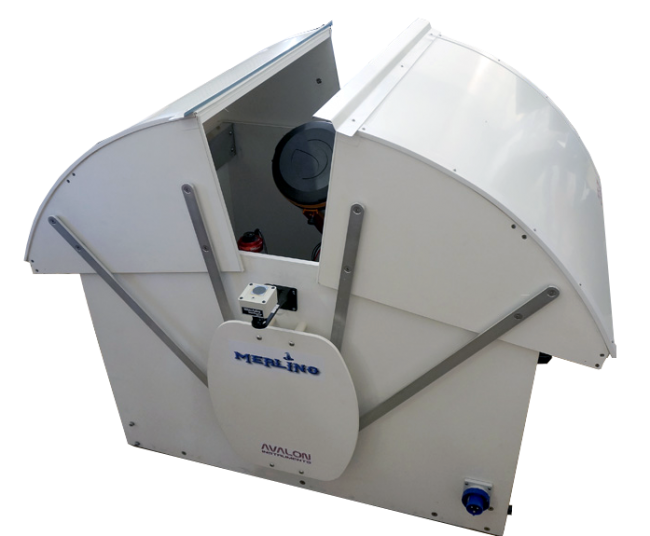
\includegraphics[width=120mm,angle=0,clip=,scale=0.7]{avalon-merlino.png}
	}
	\caption{Cupola Merlino remotizzata pronta all'uso della Avalon}
	\label{MERLINO}
\end{figure}
\`E una solutione bult-in, pronta all'uso. Il colore \`e bianco, ma \`e possibile riverniciarla in modo tale che la sua estetica sia compatibile con quella dell'ambiente che la circonda. Come \`e visibile sempre in Fig.~\ref{MERLINO}, il tetto si apre dal centro e scivola lungo i lati, rendendo minimo l'ingombro. Le sue dimensioni sono di: $1.65 mt. \times 1.20 mt. \times 1.25 mt$ che la rende una soluzione molto compatta. L'accesso al telescopio \`e garantito da una porta abbastanza robusta posta sul retro della struttura.
\\
Il costo di questa struttura \`e a partire da \textbf{14250euro} 

\subsection{Collegamento sala di controllo - telescopio}
Durante l'ultimo sopralluogo \`e stato possibile vedere che tutta la scuola \`e gi\`a cablata e predisposta per poter portare il segnale internet ai vari hot-spot distribuiti nelle varie aree. Ci hanno anche informato che internet non funziona. La rete dell'osservatorio (gi\`a strutturata a Villa Dho) \`e indipendente dal fatto che il segnale  internet ci sia o meno. Per noi \`e solo necessario che ci venga assegnato un cavo che porti il segnale dal nostro switch nella sala di controllo, allo switch situato nell'area pi\`u prossima al telescopio. Successivamente dovr\`a partire una canalina per portare il segnale dallo switch a dentro il riparo.

La nostra infrastruttura di rete \`e totalmente indipendente dal fatto che funzioni o meno quella della scuola. A noi serve solo un cavo che porti il segnale il pi\`u vicino possibile al nostro telescopio. Dal sopralluogo pare che la scuola abbia gi\`a un cablaggio ethernet strutturato a cui potersi appoggiare.





\end{document}
